\documentclass[11pt,a4paper]{ctexart}

\usepackage[margin=2.6cm]{geometry}
\usepackage{amsmath,amssymb,amsthm}
\usepackage{graphicx}
\usepackage{booktabs}
\usepackage{hyperref}
\usepackage{xcolor}
\usepackage{listings}
\usepackage{caption}

\graphicspath{{figures/}}
\hypersetup{colorlinks=true, linkcolor=blue!50!black, urlcolor=blue!60!black}
\lstset{
  basicstyle=\ttfamily\small,
  breaklines=true,
  frame=single,
  columns=fullflexible,
  backgroundcolor=\color{gray!7}
}

\newtheorem{definition}{定义}[section]
\newtheorem{theorem}{定理}[section]
\newtheorem{lemma}{引理}[section]
\newtheorem{proposition}{命题}[section]
\newtheorem{example}{例}[section]

\title{附录 B \quad Mixingales and physical dependence / Mixingales 与物理依赖}
\author{基于 \textit{A Course in Time Series Analysis} 的中文讲义与 Python 实践}
\date{}

\begin{document}
\maketitle

\section*{本章学习目标}

本章按照原文 \textit{Mixingales and physical dependence} 的小节顺序整理，保留主要定义、定理、模型公式和练习方向，并将原文中的 R 实践思路改写为 Python 工程实践。

完成本章后，应能够：
\begin{itemize}
  \item 定义 mixingale 并理解其依赖衰减含义；
  \item 获得几乎必然收敛率；
  \item 理解 Theorem 14.7.3 的证明结构；
  \item 掌握物理依赖度量；
  \item 把 ARMA 过程放入依赖衰减框架。
\end{itemize}

\section{Mixingale}

\begin{definition}[Mixingale，原文 Definition B.0.1]
设 \(\mathcal F_t\) 为过滤。若随机变量 \(X_t\) 满足对过去和未来条件期望的影响随滞后衰减，例如
\[
  \|E(X_t\mid\mathcal F_{t-m})\|_p\le c_t\psi_m,
\]
其中 \(\psi_m\to0\)，则称 \(\{X_t\}\) 为 mixingale。
\end{definition}

\begin{lemma}[分解，原文 Lemma B.0.1]
mixingale 可分解成若干近似鞅差项和可控余项，因此能使用鞅工具证明收敛。
\end{lemma}

\section{几乎必然收敛率}

\begin{lemma}[原文 Lemma B.1.1]
若随机序列 \(S_T\) 的最大二阶矩满足
\[
  E\left(\sup_{t\le T}|S_t|^2\right)\le \phi(T),
\]
则可通过分块和 Borel-Cantelli 引理得到几乎必然收敛率。
\end{lemma}

该节服务于第 14 章估计量收敛率证明：不仅要知道误差趋于 0，还要知道趋于 0 的速度。

\section{Theorem 14.7.3 的证明}

原文证明 ARMA 过程在根离单位圆条件下具有足够快的依赖衰减。若
\[
  X_t=\sum_{j=0}^{\infty}\psi_j\varepsilon_{t-j},
\]
且 \(|\psi_j|\) 几何衰减，则远过去创新对当前的影响迅速变小。

\begin{lemma}[ARMA mixingale 性质，原文 Lemma B.2.1--B.2.2]
满足因果可逆条件的 ARMA 过程可构造为 mixingale，并满足第 14 章所需的几乎必然界。
\end{lemma}

\section{物理依赖性质}

物理依赖度量把过程写成
\[
  X_t=G(\ldots,\varepsilon_{t-1},\varepsilon_t).
\]
将某个过去创新 \(\varepsilon_{t-k}\) 替换为独立副本，得到耦合变量 \(X_t^{*(t-k)}\)。依赖度量定义为
\[
  \delta_p(k)=\|X_t-X_t^{*(t-k)}\|_p.
\]
若 \(\delta_p(k)\) 快速衰减，说明遥远冲击对当前影响很小。

\begin{lemma}[原文 Lemma B.3.1]
在适当 \(p\) 阶矩和物理依赖可和条件下，可得到部分和、样本协方差和估计量所需的矩界。
\end{lemma}

\section{Python 工程实践}

在本章目录下运行：
\begin{lstlisting}[language=bash]
python scripts/appB_generate_figures.py
\end{lstlisting}

脚本会把图像写入本章 \texttt{figures/} 目录。当前图像用于配合本章核心概念的仿真说明；若后续补齐原始数据文件，可把模拟数据替换为原文真实数据案例。

\begin{figure}[htbp]
  \centering
  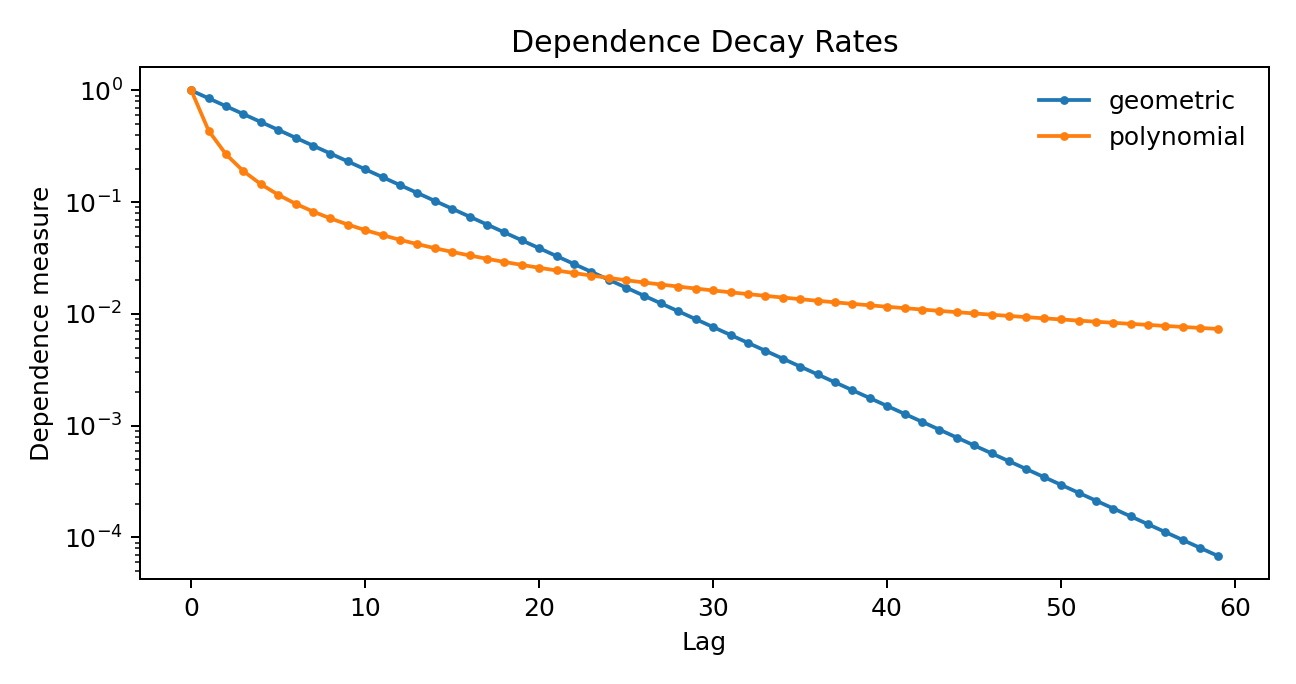
\includegraphics[width=0.86\textwidth]{appB_fig01_dependence_decay.png}
  \caption{依赖衰减率：几何衰减通常比多项式衰减带来更强的渐近结果。}
\end{figure}

\begin{figure}[htbp]
  \centering
  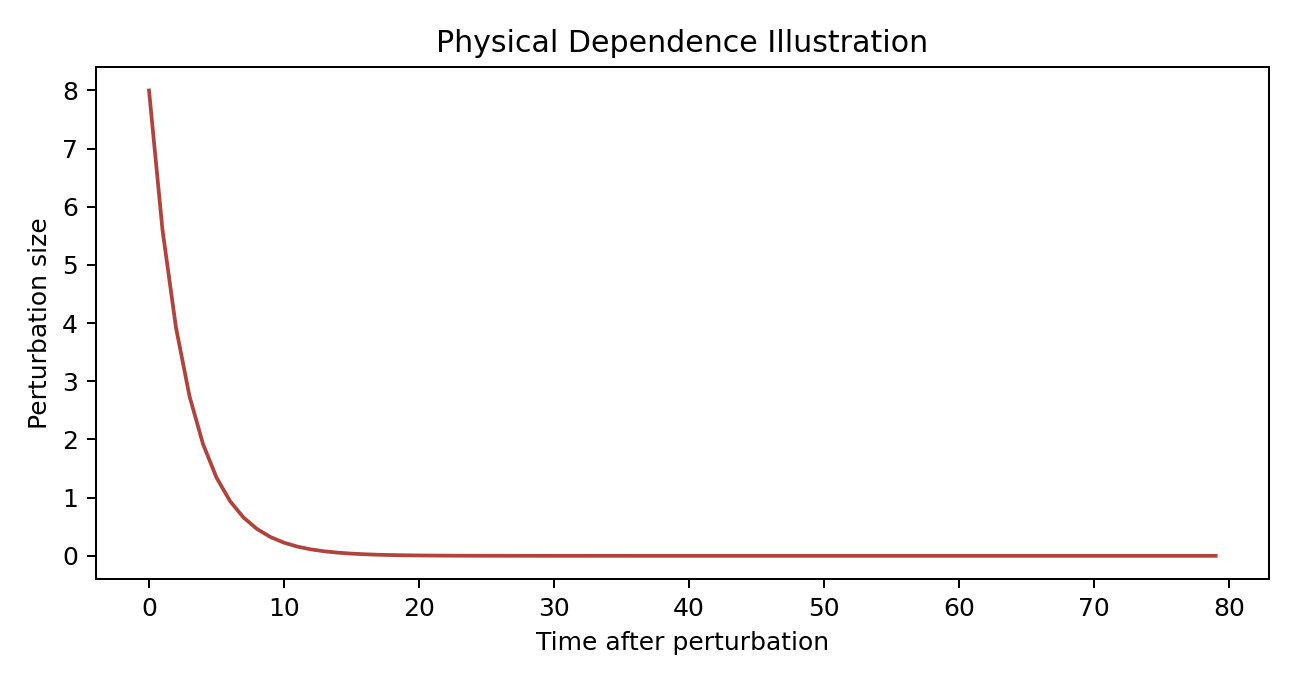
\includegraphics[width=0.86\textwidth]{appB_fig02_physical_dependence.png}
  \caption{物理依赖示意：替换一个早期冲击后，其影响随时间逐渐消失。}
\end{figure}

\section{练习提要}

原文练习主要围绕下列方向展开：
\begin{itemize}
  \item 验证简单 MA(q) 过程的 mixingale 条件；
  \item 用分块法推出几乎必然收敛率；
  \item 计算 AR(1) 的物理依赖度量；
  \item 比较几何衰减和多项式衰减对定理条件的影响。
\end{itemize}

\section*{本章小结}

附录 B 提供处理弱依赖过程的技术框架。Mixingale 和物理依赖都在量化“远处冲击影响变小”，它们是第 14 章渐近证明背后的依赖控制工具。

\end{document}
